\title{A Simple Model for Antarctic Near-Surface Index of Refraction and Radio Pulse Trajectories}
\author{Jordan C. Hanson, CCAPP, The Ohio State University}
\date{\today}
\documentclass[12pt]{article}
\usepackage[margin=2cm]{geometry}
\usepackage{amsmath,mathtools}
\usepackage{graphicx}

\begin{document}
\maketitle

\begin{abstract}
The standard model for the index of refraction in Antarctic firn is presented as a function of ice depth.  The model provides a good fit to the data, but does not account for small-scale fluctuations in snow density in the upper regions of the firn.  The standard model implies curved paths for radio pulses.  In specific situations, Fermat's principle implies that the \textit{shadowing effect} should occur.  However, data collected in the 2011-12 season in Moore's Bay directly contradicts basic shadowing. A more complete model should include surface propagation due to ray-trapping between local snow layers.
\end{abstract}

\section{A Derivation of the Density Profile}

The \textit{compressibility} $\chi$ of a simple block of material with volume $l^2\Delta z' = v$ and uniform pressure $p$ is defined as

\begin{equation}
\chi = -\frac{1}{v} \frac{\Delta v}{\Delta p}
\label{eq:comp1}
\end{equation}

Rearranging,

\begin{equation}
-\frac{\Delta v}{v} = \chi \Delta p
\label{eq:comp2}
\end{equation}

Suppose that a block comprised of snow, ice and air, known as \textit{firn}, with volume $l^2\Delta z' = v$ is compressed by a pressure $p$ originating from a force in the z-direction.  The density of the uncompressed block is $m/(l^2\Delta z')$, where $m$ is the mass.  The length of the block on the compressed side becomes $\Delta z'-\epsilon = \Delta z$, the volume decreases by $\Delta v = v_{ f} - v_{ i} = -\epsilon l^2$, and the change in density is

\begin{equation}
\Delta \rho = \rho_{f} - \rho_{\rm ice} = m \left( \frac{1}{v_{f}} - \frac{1}{v_{i}} \right) = -\frac{m\Delta v}{v_{f} v_{ i}} = -\rho_{f} \frac{\Delta v}{v}
\label{eq:deltarho}
\end{equation}

From now on, the initial volume is $v_i = v$.  Substituting Eq. \ref{eq:comp2} into Eq. \ref{eq:deltarho}, 

\begin{align}
\Delta \rho =& \rho_{f} \chi \Delta p \\
\Delta p =& \left(\chi \rho_{f}\right)^{-1} \Delta \rho
\end{align}

Dividing both sides by $\Delta z$, taking the limit $\Delta z \to 0$, and relabelling $\rho_{\rm f}$ to simply $\rho$:

\begin{align}
\frac{\Delta p}{\Delta z} =& \left(\rho_{f} \chi \right)^{-1} \frac{\Delta \rho}{\Delta z} \\
\Aboxed{p' =& \left(\chi \rho\right)^{-1} \rho'} \label{eq:note}
\end{align}

Equation \ref{eq:note} relates changes in pressure to changes in density, and it will be required for the derivation of the firn density profile.  There are three potential choices for implementing Eq. \ref{eq:note} in the firn derivations.  First, the assumption may be taken that \textit{$\left(\chi \rho\right)^{-1} = \left(\chi_0 \rho_0\right)^{-1}$ is an empirical constant} relating $p'(z)$ to $\rho'(z)$, akin to assuming constant compressibility for some average density range.  Second, the assumption may be taken that \textit{$\chi(z)$ depends on depth, and $\rho=\rho_0$ is some empirical constant}.  This assumption simplifies the following mathematics, relative to the third possibility that both factors in \textit{$(\chi(z)\rho(z))^{-1}$ depend on depth}.  The following three sections compare the implications of these assumptions.

\subsection{Firn profile, with $p'(z) = (\chi_0\rho_0)^{-1} \rho'(z)$}
\label{sec:firn1}

Let the region of firn be described by $N$ firn blocks labelled by $j$, with varying density $\rho_j$.  Let the snow surface correspond to $j=N$, $z=0$, and the beginning of solid ice (the bottom of the firn) correspond to $j=0$, $z=-h$.  Each compressed block has a height $\Delta z$, and a volume $v = l^2\Delta z$.  The normal force $f = p_{j} A$ on block $j$ must oppose the weight of block $j$, and the total mass M of the firn above block $j$:

\begin{align}
l^2 p_{j} &= g\left(m_{j} + M\right) \label{eq:force1} \\
M &= \sum_{i = j+1}^{N} m_{i} = \sum_{i = j+1}^{N} \rho_{\rm ice} l^2 \Delta z \label{eq:force2} \\
m_{j} &= \rho_{j} l^2 \Delta z \label{eq:force3}
\end{align}

Combining Eqs. \ref{eq:force1}-\ref{eq:force3}, and cancelling the common $l^2$ factor,

\begin{equation}
p_{j} = g \sum_{i = j}^{N} \rho_{\rm ice} \Delta z
\end{equation}

Take the limit $\Delta z \to 0$:

\begin{equation}
p(z) = g \int_{z}^{0} \rho(z') dz'
\label{eq:rho1}
\end{equation}

Reversing the limits of integration, and taking the derivative of both sides:

\begin{equation}
p'(z) = -g(\rho(z) - \rho(0))
\label{eq:rho2}
\end{equation}

Substituting Eq. \ref{eq:note} into Eq. \ref{eq:rho2}, assuming $(\chi_0\rho_0)^{-1}$ is some coefficient,

\begin{equation}
\rho' = -\left(g \chi_0 \rho_0\right)(\rho(z)-\rho(0))
\label{eq:rho3}
\end{equation}

Differentiating once more yields:

\begin{equation}
\rho'' = -\left(g \chi_0 \rho_{0}\right) \rho'
\label{eq:rho4}
\end{equation}

The factor in parentheses has dimensions of inverse length: $z_0^{-1} = \left(g \chi_0 \rho_{0}\right)$.  There are two boundary conditions: the surface behavior $\rho(0) = \rho_{\rm s}$, and the deep behavior $\lim_{z\to-\infty} \rho(z) = \rho_{\rm ice}$, requiring the second-order differential equation.  Letting $\Delta\rho = \rho_{\rm ice} - \rho_{\rm s}$, the following equation is a solution to Eq. \ref{eq:rho4}:

\begin{equation}
\boxed{\rho(z) = \rho_{\rm ice} - \Delta \rho \exp(z/z_0)}
\label{eq:rho5}
\end{equation}

Although the depth-scale $z_0$ of the firn is controlled by the compressibility of the firn ice $chi_0$, this relation is empirical until the compressibility depth-dependence is specified.  It is shown in Sec. \ref{sec:fit} that Eq. \ref{eq:rho5} is an excellent fit to firn data taken from around Antarctica.

\subsection{Firn profile, with $p'(z) = (\chi(z)\rho_0)^{-1} \rho'(z)$}
\label{sec:firn2}

If the compressibility $\chi=\chi(z)$ depends on depth, then Eq. \ref{eq:rho4} becomes

\begin{equation}
\rho'' = -(g\rho_0)(\chi\rho'+\chi'\rho)
\label{eq:rho6}
\end{equation}

Given that the form of Eq. \ref{eq:rho5} matches empirical data, then $\chi(z)$ may be found by solving Eq. \ref{eq:rho6}.  Inserting $\rho(z)$ and $\rho'(z)$ from Eq. \ref{eq:rho5} into Eq. \ref{eq:rho6},

\begin{equation}
\chi' = \frac{\chi z_0^{-1} + g\rho_0z_0^{-2}}{\left(\frac{\rho_{\rm ice}}{\Delta\rho}\right)e^{-z/z_0} - 1}
\label{eq:rho7}
\end{equation}

Let $y = z_0^{-1} \chi + g\rho_0 z_0^{-2}$, $\Delta\rho/\rho_{\rm ice} = q$, and $u = z/z_0$.  Equation \ref{eq:rho7} simplifies to

\begin{equation}
\frac{dy}{du} = \frac{q e^{u}}{1-q e^{u}}
\label{eq:diffrho1}
\end{equation}

This differential equation is first-order, admitting one integration constant $c_1$ in the solution:

\begin{equation}
y(u) = c_1(1-qe^u)^{-1}
\label{eq:diffrho2}
\end{equation}

Replacing variables with the original definitions,

\begin{equation}
\chi(z) = \frac{c_1z_0}{1-\left(\frac{\Delta\rho}{\rho_{\rm ice}}\right)e^{z/z_0}} - (g\rho_0z_0)^{-1}
\end{equation}

Taking the deep limit $\lim_{z\to-\infty} \chi(z) = \chi_{\rm ice}$, $c_1 = z_0^{-1}(\chi_{\rm ice}-(g\rho_0z_0)^{-1})$.  Defining the \textit{firn compressibility} $\chi_{\rm f} = (g\rho_0z_0)^{-1}$, Eq. \ref{eq:diffrho2} becomes

\begin{equation}
\chi(z) = \frac{\chi_{\rm ice}+\chi_{\rm f}}{1-\left(\frac{\Delta\rho}{\rho_{\rm ice}}\right)e^{z/z_0}}-\chi_{\rm f}
\label{eq:chi1}
\end{equation}

Notice that if the deep limit is taken, $\chi \to \chi_{\rm ice}$.  If $z = 0$, $\chi(0) = \chi_{\rm s}$ is

\begin{equation}
\rho_{\rm s} \chi_{\rm s} = \rho_{\rm ice}\chi_{\rm ice}+\Delta\rho\chi_{\rm f}
\label{eq:chi2}
\end{equation}

Equation \ref{eq:chi2} is physically intuitive.  The ice compressibility should be much smaller than than the snow compressibility ($\chi_{\rm ice} \ll \chi_{\rm s}$), in which case the firn compressibility is the snow compressibility times the fractional density change from the surface to the firn.

\subsection{Firn profile, with $p'(z) = (\chi(z)\rho(z))^{-1} \rho'(z)$}
\label{sec:firn3}
The model for compressibilty $\chi(z)$ in Sec. \ref{sec:firn2} that preserves the firn density profile found in Sec. \ref{sec:firn1} (which matches the data in Sec. \ref{sec:fit}) is physically intiuitive for several reasons.  First, it must contain the fact that snow in the upper firn is more compressible than pure ice at depths $z \ll z_0$.  Second, it fits the boundary conditions, in that the firn compressibility is a weighted difference between the surface compressibility and ice compressibility (Eq. \ref{eq:chi2}).  Third, the firn scale $z_0^{-1} = g\rho_0\chi_{\rm f}$ is shown to be proportional to the firn compressibility, $\chi_{\rm f}$.  That is, the more compressible the surface snow for a given glacier, ice sheet, or ice shelf, the smaller is $z_0$, leading to a shallower transition to solid ice.

The $\rho_0$ parameter is not yet explained, however.  It may be included in the model, provided that $p'(z) = (\chi(z)\rho(z))^{-1} \rho'(z)$.  Let $\rho(0) = \rho_{\rm s}$,  $p'(z) = (\chi(z)\rho(z))^{-1} \rho'(z)$, and insert these statements into Eq. \ref{eq:rho3}:

\begin{equation}
\rho'(z) = -g\rho^2(z)\chi(z) + g\rho(z)\rho_{\rm s}\chi(z)
\label{eq:chi3}
\end{equation}

In the same fashion as Sec. \ref{sec:firn2}, the compressibility function $chi(z)$ may be derived by asserting Eq. \ref{eq:rho5}.  The result is

\begin{equation}
\chi(z) = \frac{\chi_{\rm ice}}{ 2\cosh(z/z_0) - \left(\frac{\rho_{\rm s}}{\rho_{\rm ice}}\right) e^{z/z_0} - \left(1+\frac{\Delta\rho}{\rho_{\rm ice}}\right)  }
\label{eq:chi4}
\end{equation}

This result is very similar in behavior to Eq. \ref{eq:chi1}, as shown in Fig.

\section{Remark about the Index of Refraction Profile}

For dielectric materials like snow and ice, the index of refraction is usually approximated as a linear equation of density: $n(z) \approx 1+b\rho(z)$, and this is usually justified through expanding the Landau-Lifshitz-Looyenga equation (see below).  Thus, the index versus depth of the metamorphosis from snow to ice follows a function like

\begin{equation}
n(z) = n_{0} - n_1 e^{z/z_0}
\end{equation}

At $z=0$, $n(0) = n_s$ (snow), and as $|z| \gg z_0$, for $z<0$, $n = n_{ice}$.  Letting $\Delta n = n_{ice} - n_{s}$, the index equation becomes

\begin{equation}
\boxed{
n(z) = n_{ice} - \Delta n e^{z/z_0}
}
\label{eq:n}
\end{equation}

Notice that the compressibility of the firn (proportional to $z_0^{-1}$) influences also the steepness of the index of refraction profile.  This is true if the index is a linear function of the density.

\section{The Landau-Lifshitz-Looyenga Equation}

Let the complex dielectric constants of snow and ice be $\epsilon_i$ and $\epsilon_s$, and the dielectric constant of their mixture be $\epsilon(z)$. Further, let the two separate dielectrics each have volume fractions $v_i$ and $v_s$, with volume fractions $v_i + v_s = 1$, $\rho(z) = v_i \rho_i + v_s \rho_s$.  The Landau-Lifshitz-Looyenga equation gives

\begin{equation}
\epsilon(z) = \left( v_i \epsilon_i^{1/3} + v_s \epsilon_s^{1/3} \right)^3
\end{equation}

Let the real and imaginary parts of dielectric constants follow the notation $\epsilon = \epsilon' + i \epsilon''$, and defined the \textit{loss tangent} as $\tan\delta = \epsilon''/\epsilon'$.  Ice has a loss tangent of order $10^{-3}$ at RF frequencies, and the loss tangent of snow is smaller.  To first order in $\tan\delta_i$ and $u = v_2/v_1 < 1$, with $\alpha = (\epsilon_2'/\epsilon_1')^{1/3}$, it may be shown that

\begin{equation}
\sqrt{\Re{\epsilon(z)}} = n(z) \approx v_i^{3/2}\epsilon_i'^{1/2}(1+u\alpha)
\end{equation}

Setting $v_2 = 0$, $v_1 = 1$ (or $u=0$) reproduces the expected $n = \sqrt{\epsilon_i'}$ for pure ice.  With $\beta = 3/2 (\rho_s/\rho_i)$, $v_i^{3/2}$ is approximately

\begin{equation}
v_i^{3/2} \approx \left(\frac{\rho(z)}{\rho_i}\right)^{3/2}(1+u\beta)^{-1}
\end{equation}

Combining equations, and recalling that $\epsilon_i'^{1/2} = n_{ice}$, the result is

\begin{equation}
\frac{n(z)}{n_{ice}} \approx \left( \frac{1+u\alpha}{1+u\beta} \right) \left( \frac{\rho(z)}{\rho_i} \right)^{3/2}
\end{equation}

Expanding to first order about $\rho(z)/\rho_i = 1$:

\begin{equation}
\frac{n(z)}{n_{ice}} \approx -\frac{1}{2}\left( \frac{1+u\alpha}{1+u\beta} \right) + \frac{3}{2}\left( \frac{1+u\alpha}{1+u\beta} \right) \frac{\rho(z)}{\rho_i}
\end{equation}

Using $n_s = \epsilon_s'^2 = 1.3$, $n_i = \epsilon_i'^2 = 1.78$, $\rho_s = 0.4$ g/cc, $\rho_i = 0.917$ g/cc, and $u=0.1$ as an example, a linear equation for the index versus density near the firn/ice boundary layer is

\begin{equation}
\frac{n(z)}{n_{ice}} \approx -0.51 + 1.66 \rho(z) [g/cc]
\end{equation}

\section{Fitting the Firn Model to the Data}
\label{sec:fit}

Many analyses and derivations have been done to produce the index of refraction versus depth curve in different locations throughout Antarctica.  Figure \ref{fig:fig1} contains a summary of such measurements.  In the figure, the function $n(z) = A-B\exp(Cz)$ is fit to the data points.  Where density data was available, the empirical conversion of $n(z) = 1.0 + 0.86\rho(z)$ has been used.

\begin{figure}[ht]
\centering
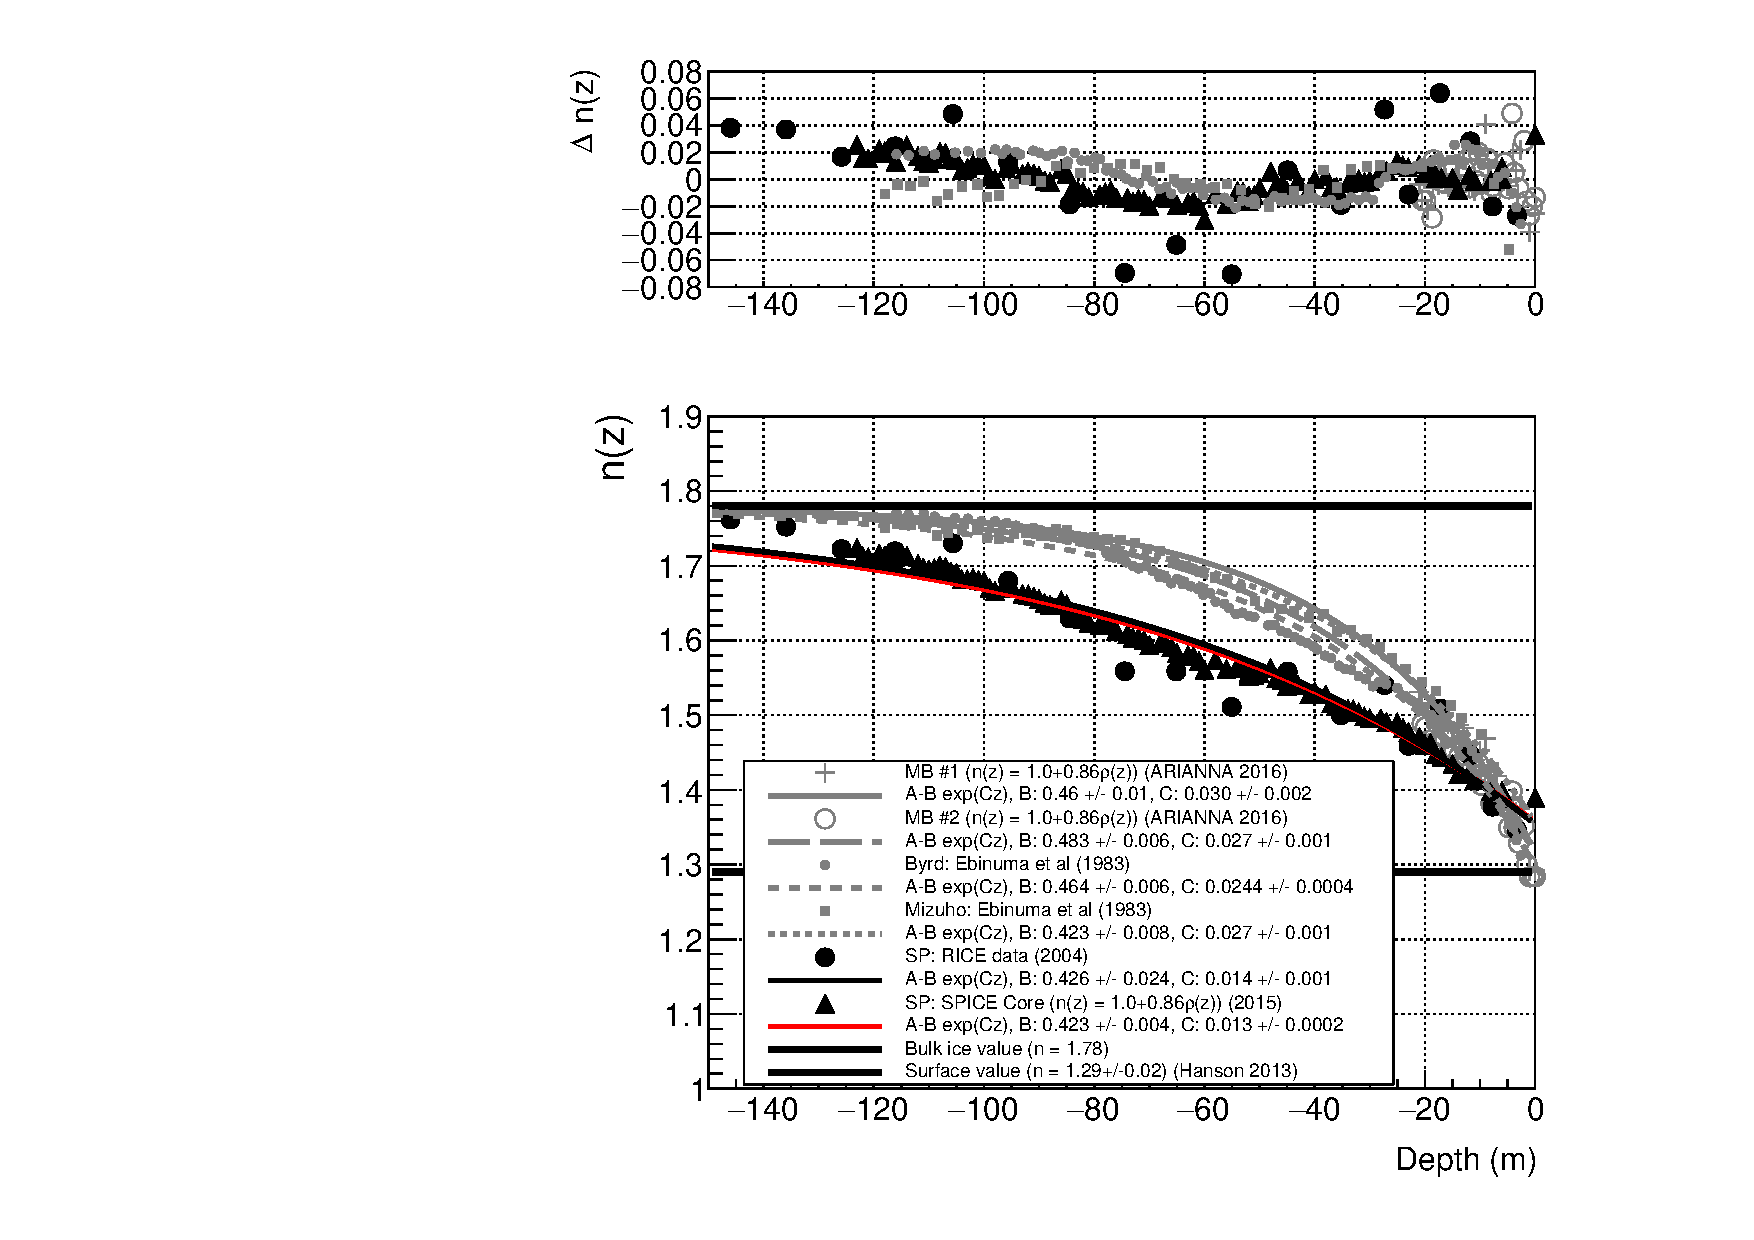
\includegraphics[width=0.6\textwidth]{figures/January17_plot1.pdf}
\caption{\label{fig:fig1} A summary of all the $n(z)$ data discovered for various locations in Antarctica, including Moore's Bay (MB) and the South Pole.  All data points and fit lines that are black correspond to the South Pole, and the gray points and fit lines correspond to Moore's Bay, Byrd station, and Mizuho station.}
\end{figure}

\begin{figure}[ht]
\centering
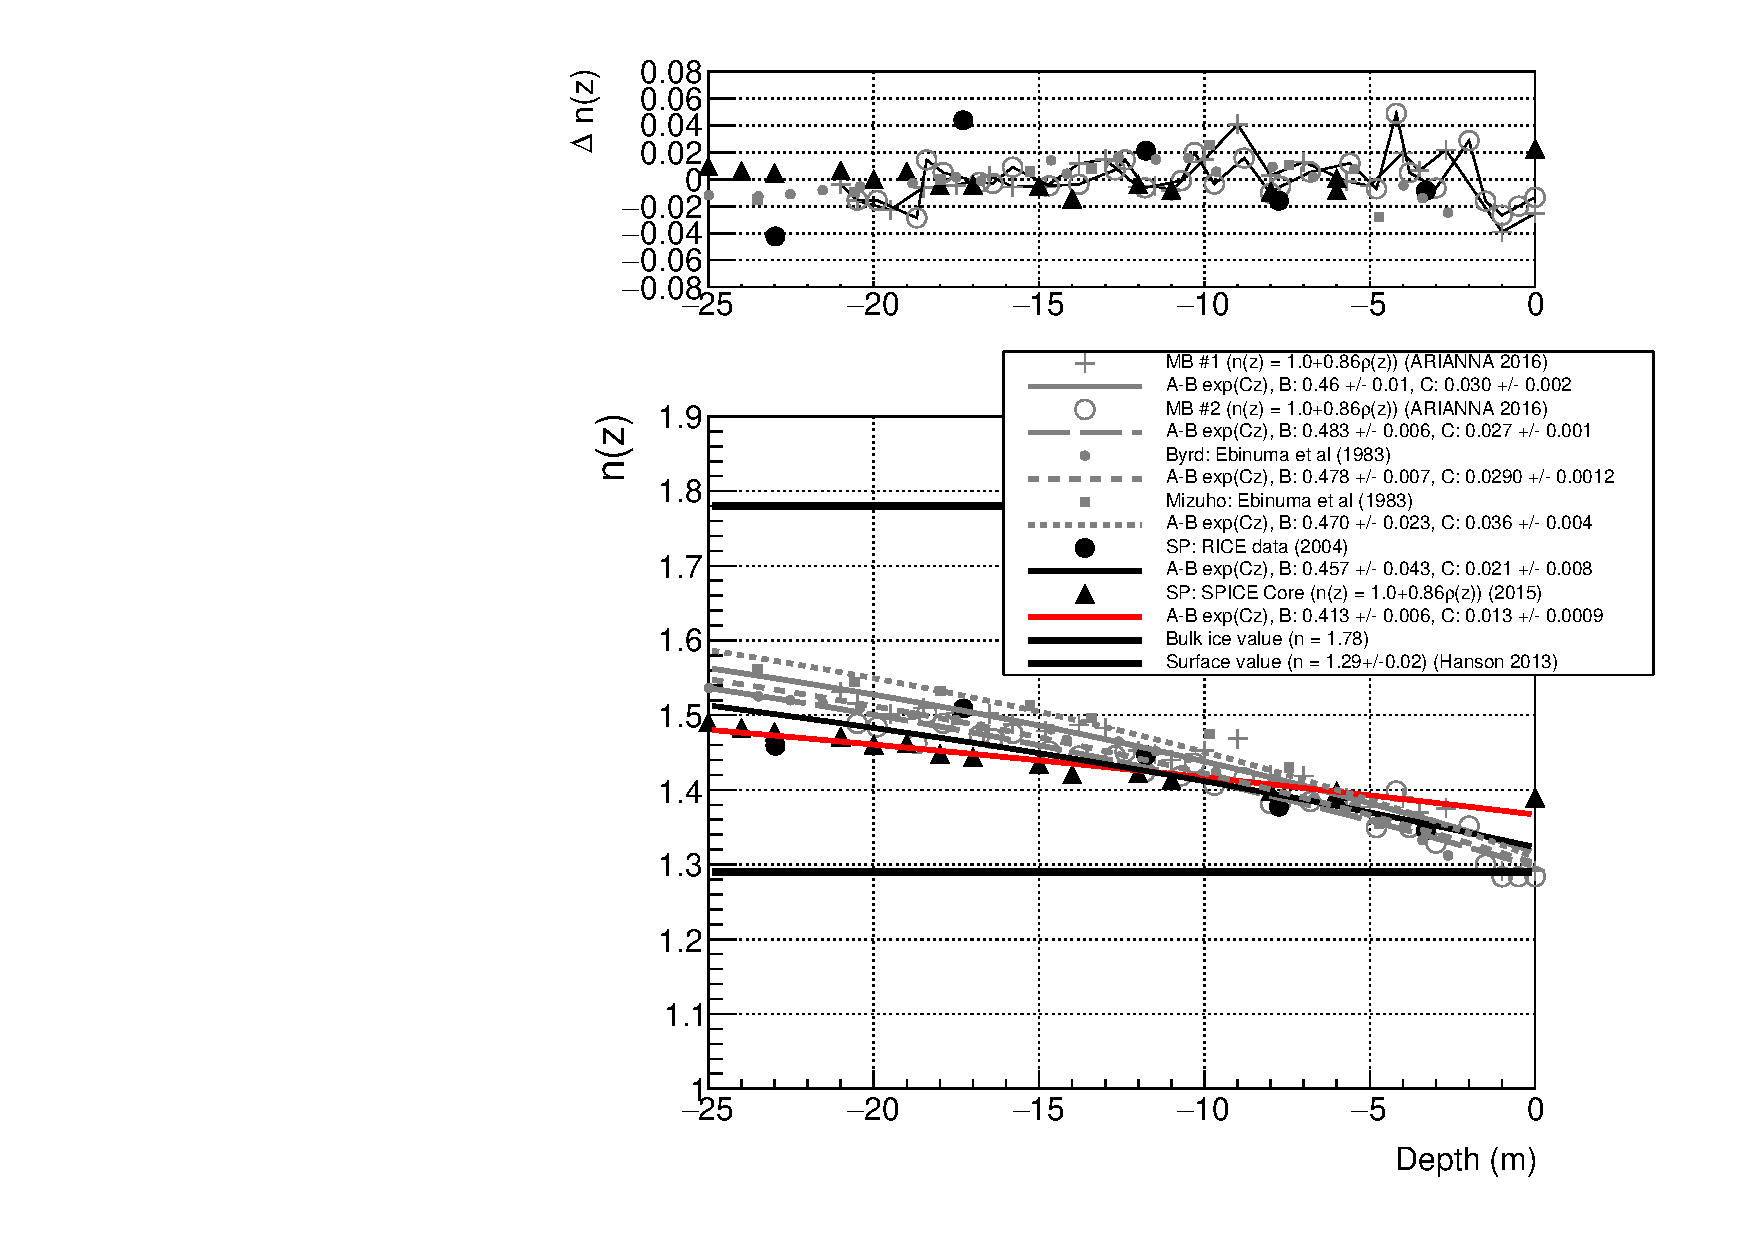
\includegraphics[width=0.6\textwidth]{figures/January17_plot2.pdf}
\caption{\label{fig:fig1a} Figure \ref{fig:fig1}, focusing on the upper few meters.}
\end{figure}

The value for $A$ in all the fits was restricted to $n_{ice} = 1.78$, from the differential equation solution to the gravity-density problem.  No restriction was placed on the value for $B=\Delta n$, but note that the results are close to $1.78-1.29 = 0.49$, where $1.29$ is the expected value for $n_s$ (Hanson 2013).  Thus, the fits are all measuring $n_s$ accurately.  The slopes $C = z_0^{-1}$ differ across the Antarctic continent, and are statistically lower at the South Pole compared to other locations.

Table 1 summarizes the results for the fits to the points in the figure.  The snow surface index of refraction is derived from the $B$ parameter, assuming $A = n_{ice}$, and $B = \Delta n = n_{ice} - n_s$.  These results may be compared to resuts from the upper 2 m ($n_s = 1.29\pm0.02$), obtained at the Ross Ice Shelf via multiple tecniques (Hanson 2013).  The curves MB\#1 and MB\#2 refer to two cores drilled in Moore's Bay (Ross Ice Shelf) in 2016, and the references for the rest of the data may be found in the Table.

Note that the Schytt model quoted by (Hanson 2015) found that $q = z_0 = 35.4$ m, which is in agreement with the MB data.  The Schytt model in (Hanson 2015) was fit to firn density data collected near Williams Field on the Ross Ice Shelf.  For index data derived from density data, the snow/ice conversion $n(z) = 1.0 + 0.86\rho(z)$ was used (ref).  The data from Ebinuma (1983) was originally quoted as pressure in kPa vs. depth, which has been converted to density via the simple formula in Shumskiy (1960):

\begin{multline}
z = \left( \frac{p-p_0}{\rho_i g}\right) \left \lbrace 1-\chi\left(\frac{p+p_0}{2} - p_n \right) \right \rbrace (1+\alpha_i\theta) \\ + \left \lbrace \frac{1}{\rho_0 g}-\frac{1-\chi(p_0-p_n)}{\rho_i g} \right \rbrace p_0 \ln (p/p_0) (1+\beta_a\theta)
\end{multline}

The parameters in the equation of depth, $z$, versus pressure, $p$, are as follows: $p_0$ is the pressure at the surface, $\rho_{\rm ice}$ is the density of ice (0.91670 g/cc) at a pressure $p_n=1$ atmosphere and a temperature $\theta = 0^{\circ}$ C, with a  volumetric compressibility of $\chi = 1.2 \times 10^{-5}$ bar$^{-1}$, a coefficient of linear expansion of $\alpha_i = 5.1 \times 10^{-5}$ C$^{\circ -1}$, and surface density of $\rho_0$.  A value of $94.306$ kPa is chosen for the surface pressure, corresponding to an altitude of $\approx 0.5$ km.  The temperature $\theta$ is the average temperature through the firn, taken to be $-10$ C$^{\circ}$ in Fig. 1 (Hanson dissertation).

\begin{table}[ht]
\centering
\begin{tabular}{| c | c | c | c | c | c |}\hline
Ref./Location & $A=n_{ice}$ & B  & $n_s$ & C (m$^{-1}$) & $z_0$ (m)\\ \hline
MB\#1/Moore's Bay & 1.78 & $0.44\pm0.01$ & $1.34\pm0.01$ & $0.038\pm0.002$ & $26\pm1$ \\ \hline
MB\#2/Moore's Bay & 1.78 & $0.458\pm0.007$ & $1.322\pm0.007$ & $0.033\pm0.002$ & $30\pm2$ \\ \hline
Ebinuma (1983)/Byrd & 1.78 & $0.464\pm0.006$ & $1.316\pm0.006$ & $0.0244\pm0.0004$ & $41\pm1$ \\ \hline
Ebinuma (1983)/Mizuho & 1.78 & $0.423\pm0.008$ & $1.357\pm0.006$ & $0.027\pm0.001$ & $37\pm1$ \\ \hline\hline
RICE (2004)/South Pole & 1.78 & $0.43\pm0.02$ & $1.35\pm0.02$ & $0.014\pm0.001$ & $71\pm5$ \\ \hline
%Eisen (2003)/South Pole & 1.78 & $0.48\pm0.01$ & $1.3\pm0.01$ & $0.020\pm0.001$ & $50\pm2.5$ \\ \hline
%Gow (xxxx)/South Pole & 1.78 & $0.435\pm0.01$ & $1.345\pm0.01$ & $0.016\pm0.001$ & $62.5\pm4$ \\ \hline
SPICE (2015)/South Pole & 1.78 & $0.410\pm0.008$ & $1.370\pm0.008$ & $0.019\pm0.0005$ & $53\pm1$ \\ \hline
\end{tabular}
\caption{\label{tab:tab0} The fit parameters for the curves shown in Fig. 1.  The function fit to the data is $n(z) = n_{ice} -\Delta n \exp(Cz)$.  The differential equation derived in the first section requires $n_{ice} = 1.78$ and $B = \Delta n = n_{ice} - n(0)$ as boundary conditions.}
\end{table}

\section{Fermat's Principle, and Ray-Tracing}

A key question for ARA/ARIANNA future designs is the expected path of a radio pulse from an Askaryan event in firn.  Beginn with Fermat's principle, which states that a ray must traverse the path that minimizes the travel time.  Fermat's principle is similar to the principle of least-action, in which a massive particle takes the path of least-resistance (cite Wiki Fermat's).

\begin{align}
\delta S &= 0 \\
\delta &\int_A^B n(z)(1+\dot{y}^2)^{1/2} dx dy dz = \delta \int_A^B L(z,\dot{y}) dx dy dz = 0
\end{align}

Derivatives indicated by the dot notation are with respect to $z$, not time.  The assumption that $x = \dot{x} = 0$ has been taken without loss of generality.  Note that $\dot{y} = dy/dz$ is unit-less, and $\ddot{y}$ has units of inverse meters.  Using the Euler-Lagrange equations to minimize the variation in the path, and letting $u = \dot{y}$:

\begin{align}
\frac{d}{dz} \left( \frac{\partial L}{\partial \dot{y}} \right) - \left( \frac{\partial L}{\partial y} \right) &= 0 \\
\frac{d}{dz} \left( \frac{\partial L}{\partial \dot{y}} \right) &= 0 \\
\dot{u} &= - \left( \frac{\dot{n}}{n} \right) (u^3+u) \label{eq:main}
\end{align}

Note that the units are inverse meters on each side of the equation: all factors of $u$ are unit-less, and $\dot{n}$ has units of inverse meters.  Putting in the model for $n(z)$, the final equation of motion is

\begin{equation}
\boxed{
\dot{u} = z_0^{-1} \left( \frac{\Delta n e^{z/z_0}}{n_{ice} - \Delta n e^{z/z_0}} \right) (u^3+u)
}
\end{equation}

As a check, note the deep ice limit: $|z| \gg z_0$, $z<0$:

\begin{equation}
\dot{u} = 0
\end{equation}

The solution to this equation of motion, after solving for $z$ is 

\begin{equation}
z(y) = a+by
\end{equation}

In other words, if the rays are far from the firn, the rays must propagate in straight lines.  For the case of a shallow ray $z \rightarrow 0$, propagating initially with a horizontal velocity component satisfying $u^3 \gg u$, the main equation of motion reduces to 

\begin{equation}
\frac{du}{dz} = \left( \frac{n_{ice} - n_s}{z_0 n_s}\right) u^3
\end{equation}

This is a variables-separable differential equation.  Using an initial point of $(y_1,z_1)$, a particular solution is

\begin{equation}
z(y) = -\frac{1}{2z_0} \left( \frac{n_{ice} - n_s}{n_s}\right) (y-y_1)^2 + z_1
\end{equation}

Thus, for a very shallow ray, with initial horizontal velocity, the solution dictates that the shortest travel time between two near-surface points is given by a quadratic path.  As an example, use $z_0 = 37$ m and $n_s = 1.30$ to describe Moore's Bay refraction, and $z_0 = 71$ m, $n_s = 1.33$ to describe the South Pole refraction.  Figure 2 compares the hypothetical ray-paths for these two cases.

\begin{figure}
\centering
\includegraphics[width=0.6\textwidth,angle=270]{figures/Jan24_plot1.eps}
\caption{\label{fig:quad} Examples of quadratic ray-paths in media with index of refraction profiles with the form of Eq. \ref{eq:n}.  The gray line corresponds to Eq: \ref{eq:n} with $z_{\rm 0} = 71$ m, and the black line corresponds to Eq: \ref{eq:n} with $z_{\rm 0} = 37$ m.}
\end{figure}

The next least-restrictive approximation for the shallow depth of the ray is $\exp{z/z_0} \approx 1+z/z_0$, rather than $z \rightarrow 0$.  Let $q = \Delta n/z_0$.  The final solution with this limit is

\begin{align}
z(y) &= -\frac{1}{2}\frac{Q_1}{z_0}(y-y_1)^2 - \frac{Q_0}{Q_1}z_0 \\
Q_1 &= 1+\frac{n_{ice}}{n_s} \\
Q_0 &= \frac{z_1}{z_0} + 1 + \frac{n_{ice}}{\Delta n}\left(\ln\left(\frac{n_s}{\Delta n}\right)-2\right)
\end{align}

Note that, in either the limit of $z \rightarrow 0$, or $\exp{z/z_0} \approx 1+z/z_0$, the solutions are quadratic, with curvature controlled by $z_0^{-1}$.  That is, if $z_0$ increases, the concavity of the ray path, and thus, the level of shadowing, decreases.  It is fascinating that the same snow metamorphosis that controls the compaction from snow to ice through gravity also controls the amount of ray bending, and that this number is measurable from the density variation versus depth.

\section{Horizontal and Near-Surface Propagation}

Thus far, the index of refraction versus depth has been treated as a smooth function.  However, perturbations from the smooth profile are introduced by variable yearly weather patterns (cite).  Over-densities and under-densities can lead to local minima and maxima in the index of refraction profile.  Let one such local under-density be described by a quadratic perturbation from what is otherwise an approximately constant $n_{\rm 0}$ value:

\begin{align}
n(z) &= n_0 - a(z-z_0)^2 \label{eq:perturb} \\
\dot{n} &= -2a(z-z_0) \\
q &= z-z_0
\end{align}

Solve Eq. \ref{eq:main} with Eq. \ref{eq:perturb}, near $q=0$ and neglecting terms up to order $q^2$, the variables-separable differential equation may be solved:

\begin{align}
\frac{du}{dq} &\approx \left(\frac{2aq}{n_0}\right) u^3 \\
\frac{dq}{dy} &\approx \pm \sqrt{-2\left(\frac{a}{n_0}\right) q^2 + C_0}
\end{align}

Choosing $C_0$ merely restricts the phase of what will become the phase of the signal.  The phase of the signal is not important under the assumption that the index profile does not depend on the horizontal coordinate.  In Monte Carlo codes this assumption may be relaxed.  Thus,

\begin{align}
\frac{dq}{dy} = &\approx \pm i \sqrt{2\left(\frac{a}{n_0}\right)}q \\
\omega^2 &= 2 \left(\frac{a}{n_0}\right) \\
\frac{dq}{dy} &= \pm i\omega q \label{eq:SHO}
\end{align}

Equation \ref{eq:SHO} admits harmonic solutions, and the spatial frequency $\omega$ is controlled by the size of the perturbation $a$ relative to the local $n_0$ value:

\begin{equation}
q(y) = A\exp(i\omega y) + B\exp(-i\omega y)
\end{equation}

The problem may also be worked with an over-density in the index of refraction profile, and the problem is the same up to an overall minus sign.  In Eqs. \ref{eq:SHO1}-\ref{eq:SHO2}, $\omega_{-}$ corresponds to an under-density $n(z) = n_0 - aq^2$, and $\omega_{+}$ corresponds to an over-density $n(z) = n_0 + aq^2$:

\begin{align}
\frac{dq}{dy} &= \pm i\omega_{-} q \label{eq:SHO1} \\
\frac{dq}{dy} &= \mp i\omega_{+} q \label{eq:SHO2}
\end{align}

\end{document}
